%! Author = t.kramer
%! Date = 15/09/2024

% \pagebreak
\section{Case study}
\label{sec:case-study}

% boundary conditions
To evaluate spatial thermal autonomy for different thermal zone sizes and passive design levels, we performed a building performance simulation case study using EnergyPlus \citep{crawley_energy_plus_2001} and Honeybee \citep{sadeghipour_roudsari_ladybug_2013}. We focus on individual spaces in a typical office building in Sydney, Australia, and use two weather files: a typical meteorological year (TMY) and a future weather file for the year 2070 (RCP 4.5) provided by the Commonwealth Scientific and Industrial Research Organisation (CSIRO), Australia \citep{ren_projected_2021}.

% simulation settings
We modeled single thermal zones with typical office configurations using US Department of Energy (DOE) reference vintages and operational programs. To capture a range of building characteristics, we tested three zone sizes (30, 60, and 180 m$^2$) and three envelope construction scenarios — Standard, Medium, and Advanced — that differed in envelope properties such as U-values, window-to-wall ratios (WWR), and shading strategies (refer to \Cref{tab:sim-settings}).


\begin{figure}[!h]
    \centering
    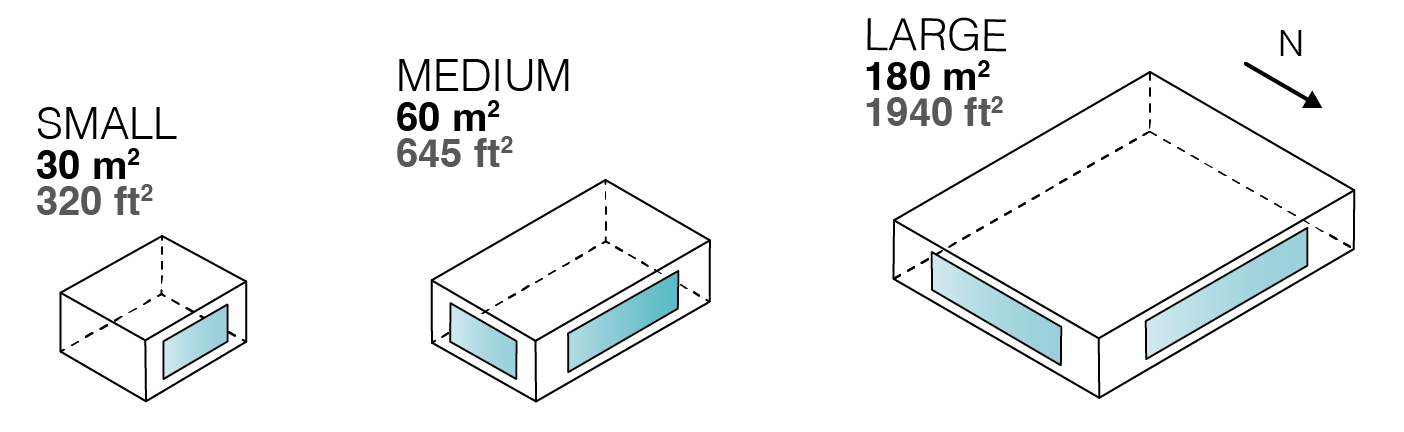
\includegraphics[width=0.8\textwidth]{manuscript/src/figures/scenario-size.png}
    \vspace{0.5cm}
    % \caption{Geometry of case study model.}

        \renewcommand{\arraystretch}{1.25}
    

        \begin{tabular}{ p{3.5cm} p{2cm} p{2cm} p{2cm} }
        
            \hline
            
            {\textbf{Setting(s)}} & \multicolumn{3}{l}{\textbf{Definition}} \\
        
            \hline
        
            {Climates}  & \multicolumn{3}{l}{Sydney, Australia (Cfa), TMY \& 2070 (RCP 4.5)} \\
        
            % \cline{2-3}
            
            {Constructions} & \multicolumn{3}{l}{\textit{ASHRAE 90.1 2019, IECC 2021}, Steel-framed*} \\
        
            % \cline{2-3}  
            
            {Program} & \multicolumn{3}{l}{\textit{Small Office*}} \\
            
            % \cline{2-3}
        
            {HVAC system} & \multicolumn{3}{l}{IdealAir system, Air conditioned} \\
        
            % \cline{2-3}

            {Passive Design Level} & {a) \textbf{Standard}} & {b) \textbf{Medium}} & {c) \textbf{Advanced}} \\

            \cline{2-4}
        
            {Natural Ventilation?} & {No} & {Yes} & {Yes} \\
        

            {Envelope} & {$U_{win} = 2.0$\newline $U_{wall} = 0.35$\newline $WWR = 0.4$ \newline No shading} & {$U_{win} = 1.3$\newline $U_{wall} = 0.2$\newline $WWR = 0.3$ \newline No shading} & {$U_{win} = 1.3$\newline $U_{wall} = 0.2$\newline $WWR = 0.3$ \newline Ext. shading} \\

             % \cline{2-3}
        
            {AC* setpoint range\newline \textit{Heating - Cooling}} & {22-24\degree C} & {22-24\degree C} & {22-24\degree C} \\
            
            \hline
        
        \end{tabular}
        \vspace{0.5cm}
        \caption{Overview of main settings for simulated case study scenarios: Construction properties, loads and schedules were based on Department of Energy (DOE) reference building information. (AC* - Air Conditioning (if used), WWR - Window-to-Wall-Ratio, U - U value in W/m²K)}
        \label{tab:sim-settings}
        

\end{figure}

For each combination of zone size and construction standard, we performed an annual thermal simulation. In addition, using the same model and based on a spatial mapping algorithm developed by \citet{mackey_2015}, we computed spatially resolved mean radiant temperature (MRT) values on a 1-meter by 1-meter grid across the zones. We then ran the simulations model both passively to calculate spatial Thermal Autonomy (sTA) and with active conditioning to assess energy use for each scenario.

To assess the impact of different thermal comfort criteria on sTA (see \Cref{eq:sta-annual}), we evaluated three hourly indices: PMV, the adaptive model, and an empirical model. The empirical model is derived from field data in the ASHRAE Global Thermal Comfort Database II \citep{foldvary_licina_development_2018,parkinson_ashrae_2022}. For this, we filtered the data to include only samples where the occupants expressed a thermal preference of 'No change' and identified the equivalent operative temperatures within the 10th to 90th percentile. This produced a comfort range of 21-28°C, which we applied as the target "comfort" range in the empirical model.

Furthermore, to evaluate spatial thermal heterogeneity in the scenarios tested, we developed a thermal heterogeneity index (THI). Similarly to sTA, we define two versions: THI$_a$ or THI$_{area}$ (\Cref{eq:thi-area}), which captures the hourly heterogeneity throughout the zone, and THI$_p$ or THI$_{point}$ (\Cref{eq:thi-point}), which summarizes the annual temperature variations at individual points on the grid. In both cases, we used the median value to derive a single-value index.

\begin{equation}\label{eq:thi-area}
    THI_a = \text{median}\left( \max_{n}(T_{n,t}) - \min_{n}(T_{n,t}) \right)
\end{equation}

\textbf{Where:}
\begin{itemize}
    \item $T_{n,t}$ is the temperature at spatial location $n$ and time $t$.
    \item $\max_{n}(T_{n,t})$ is the maximum temperature across locations $n$ at each hour $t$.
    \item $\min_{n}(T_{n,t})$ is the minimum temperature across locations $n$ at each hour $t$.
\end{itemize}

\begin{equation}\label{eq:thi-point}
    THI_p = \text{median}\left( \max_{t}(T_{p,t}) - \min_{t}(T_{p,t}) \right)
\end{equation}

\textbf{Where:}
\begin{itemize}
    \item $T_{p,t}$ is the temperature at point $p$ and time $t$.
    \item $\max_{t}(T_{p,t})$ is the maximum temperature across time $t$ (over the year) for each point $p$.
    \item $\min_{t}(T_{p,t})$ is the minimum temperature across time $t$ (over the year) for each point $p$.
\end{itemize}

\vspace{0.25cm}

Lastly, to aid post-processing and analyze and visualize spatial indoor data, we developed a array-based Python module called comfortSIM. Custom functions in comfortSIM help to explore spatial thermal heterogeneity, calculate sTA based on various thermal comfort indices from the pythermalcomfort package \citep{tartarini_pythermalcomfort_2020}, and evaluate the resilience of the building during passive operation by looking at the hourly temperature distribution across the thermal zone. The beta version of comfortSIM used for the analysis is openly accessible on \href{https://github.com/t-kramer/comfortSIM}{GitHub}.

